\subsection{Matrix Factorization Models} \label{bg:sub:factorizationmodels}
%Function
Matrix Factorization Model methods are dimensionality reduction techniques used for recommendation that generally find latent features for items, and the propensity for users towards each latent feature. This also helps with finding nontrivial correlations in the data as a latent feature could be something that is not at all obvious, but is really important.
Matrix Factorization (MF) makes an approximation of a matrix of ratings by decomposing it into multiple matrices. Since MF approximates matrices in an offline step before recommendation, it scales better compared to contemporary Collective Filtering techniques during recommendation. It performs well even when data sparsity is a concern due to the matrix approximation and the dimensionality reduction.
As data sparsity grows in a set, the less accurate every method gets. Factorization methods counteract this by compressing the data, making it less sparse, and easier to cluster.
As an MF matrix is traditionally updated offline resulting in unchanging matrices, then the matrix can be reused as required. This is a benefit when testing various aggregations or configurations of users.

\subsubsection{Singular Value Decomposition}
Commonly referred to by its acronym, SVD, was popular during Netflix's movie recommender contest amongst the top performing entrants.

On its own, SVD is a dimensionality reduction technique. However in 2006 Simon Funk \cite{svdsimonfunk} popularized it as a recommender method with some modifications.

Given a matrix of user ratings, SVD works by decomposing the matrix as seen in equation \ref{eq:svd_decomp} into two matrices called the left and right singular vectors, $U$ and $V$ respectively, and a matrix holding the singular values on its diagonal, $\Sigma$, as per the SVD theorem\cite{svdtheorem}. For this example, the left singular vector would hold the users on one side, and their inclination towards each latent feature. The right vector would conversely hold all the rated items, and their inclination towards each latent feature.

\begin{equation} \label{eq:svd_decomp}
\centering
M = U\times \Sigma \times V^T
\end{equation}

SVD considers as many features as there are ranks, but not all of them are influential. Reducing the number of features to consider is trivial, as the largest singular values stored in $\Sigma$ have the most influence.

At this point, it is possible to find some interesting similarities among the users, however to use SVD for recommendation, we must account for the missing ratings. By slightly tweaking the equation, as seen in \ref{eq:svd_AB_squeezing}, we get an A and B matrix, holding users and items respectively. This is results in three matrices looking like \ref{fig:svd_squeeze}\todo{Fix ref to figure below}.

\begin{equation}\label{eq:svd_AB_squeezing}
	\centering
	U\times \Sigma \times V^T = U\Sigma^{1/2} \Sigma^{1/2}V^T = AB
\end{equation}

\begin{figure} [H] \label{fig:svd_squeeze}
	\centering
	\includegraphics[scale=0.75]{svd_ab_squeeze.png}
	\caption{The decomposition of a rating matrix using SVD}
\end{figure}
\todo{Temporary figure from course slides - replace with own - F as features instead of K}

Having moved to the dense subspace of each rated item and user being defined by their features rather than their explicit ratings, data sparsity becomes less of a problem, as missing ratings are squeezed out.

\subsubsection{Gradient descent}
In Funk's blog, the gradient descent optimization algorithm is proposed as a common method to learn the A and B matrices to minimize the error, as found using Equation \ref{eq:gradient_descent_error}. The error is calculated as the euclidean distance between our known ratings, $R$, and our predicted ratings $\hat{R}$.

\begin{equation}\label{eq:gradient_descent_error}
\text{Error} = |R-\hat{R}| = |R - AB| = \sum_{u=1}^{U}\sum_{i=1}^{I}\left (R_{ui}- \sum_{k=1}^{K} A_{uk}B_{ki} \right )^2
\end{equation}

Given as a function, the gradient will point in the direction of the largest error increase, as shown in equation \ref{eq:derivative_gradient}. So to minimize the error, steps are taken towards the negative of the gradient.

\begin{equation}\label{eq:derivative_gradient}
	\begin{split}
	\frac{dError}{dA}=-(R-AB)B^T = \sum_{i=1}^{I}(R_{ui} - \sum_{n=1}^{N} A_{un}B_{ni})B_{ki}
	\\
	\frac{dError}{dB}=-(R-AB)A^T = \sum_{u=1}^{U}(R_{ui} - \sum_{n=1}^{N} A_{un}B_{ni})A_{uk}
	\end{split}
\end{equation}

Taking the average error when finding the derivative is a costly operation for learning the A and B matrices, as it sums up the error for every user-item pair across all of their features. This can be expressed by a running time as shown in equation \ref{eq:gradient_descent_runningtime}.

\begin{equation}\label{eq:gradient_descent_runningtime}
	\Theta(U\times I \times K)
\end{equation}

The common solution is using the stochastic gradient descent. For this, a single observed rating is selected at random for each update step of the gradient descent, rather than summing up over all the item-user pairs to find the exact gradient. The updates will be a bit more erratic, but will overall tend towards the gradient, as seen in figure \ref{fig:gradient_descent}.

\begin{figure}\label{fig:gradient_descent}
	\centering
	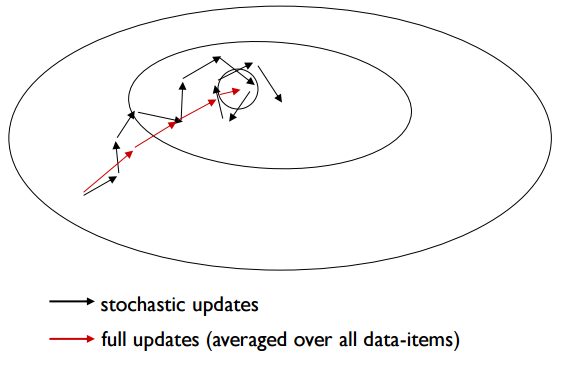
\includegraphics[scale=0.5]{gradient_descent.png}
	\caption{Gradient descent comparison with the stochastic variant as they move towards the gradient}
\end{figure}

The learning rate describes the speed at which the gradient descent changes at each step. A high learning rate will mean fewer steps and a lower chance of getting stuck in a local minimum, however a high learning rate makes convergence more difficult as the model can end up dancing around the minimum by taking too large steps near the end. A too small learning rate can result in the model settling in a local minimum for the cost function, unable to escape, as the gradient of the error will always point back towards the nearest local minimum. A learning rate is usually between $0.1$ and $0.001$, but it is recommended to take an exploratory approach. In equation \ref{eq:matrixfactorization_learningrate}, $\eta$ is the learning rate.

\begin{equation}\label{eq:matrixfactorization_learningrate}
	\begin{split}
	A_{uk}\leftarrow A_{mk} + \eta(R_{ui}-\sum_{n=1}^{N}A_{un}B_{ni})B_{ki}
	\\
	B_{ki}\leftarrow B_{ki} + \eta(R_{ui}-\sum_{n=1}^{N}A_{un}B_{ni})A_{uk}
	\end{split}
\end{equation}

Regularization helps avoid overfitting, where a model fits its training data too closely so that it predicts extremely well but only within the training data. It is added as an additional modifier when updating the model as can be seen in equation \ref{eq:matrixfactorization_regularization}, where $\lambda$ is the regularization value. It makes the resulting model more general, which improves accuracy when moving beyond the training set.

\begin{equation}\label{eq:matrixfactorization_regularization}
	\begin{split}
	A_{uk}\leftarrow A_{mk} + \eta(R_{ui}-\sum_{n=1}^{N}A_{un}B_{ni})B_{ki}-\lambda A_{uk}
	\\
	B_{ki}\leftarrow B_{ki} + \eta(R_{ui}-\sum_{n=1}^{N}A_{un}B_{ni})A_{uk} -\lambda B_{ki}
	\end{split}
\end{equation}

\subsubsection{Non-negative Matrix Factorization}

Non-negative Matrix factorization is a constraint on the usual matrix factorization. All values are equal to 0 or higher, and always positive, and when learning the model, no values will dip below 0. This is helpful for speeding up the learning in certain use cases, for instance finding objects or parts hereof in images \cite{nnmf}.

As shown in Equation \ref{eq:nmf}, given a rating matrix of size \textit{m-by-n}, for example m users and n items, we can find non-negative matrix factors $W$ and $H$ of size \textit{m-by-k} and \textit{k-by-n} such that they approximate $V$.

\begin{equation} \label{eq:nmf}
	V \approx W H
\end{equation}

%http://www.kyb.mpg.de/fileadmin/user_upload/files/publications/attachments/CFEMF_KDDW2007_4614[0].pdf